\documentclass[12pt]{article}

\usepackage{fullpage}
\usepackage{multicol, multirow}
\usepackage{tabularx}
\usepackage{standalone}
\usepackage{listings}
\usepackage{ulem}
\usepackage{amsmath}
\usepackage{pdfpages}
\usepackage[utf8]{inputenc}
\usepackage[russian]{babel}

\newcommand{\StudentName}{Ильвохин Дмитрий}
\newcommand{\Group}{1O-106М}
\newcommand{\CourseName}{Обработка естественных языков}
\newcommand{\LabNum}{1}
\newcommand{\Subject}{Закон Ципфа}
\newcommand{\PrepName}{Калинин А.\,Л.}

\begin{document}

\lstset
{
        language=Python,
        basicstyle=\footnotesize,% basic font setting
        extendedchars=\true
}

\begin{flushright}
\Large{
	\CourseName \\
	Лабораторная работа №\,\LabNum \\
	<<\Subject>> \\
  \StudentName, \Group \\
  Дата: \line(1,0){150} \\
  Подпись: \line(1,0){150} \\
}
\end{flushright}

\subsection*{Задание}
Построить зависимость частоты слова от позиции в отсортированной
по убыванию частоты последовательности слов.

Подобрать коэффициенты $const$, $\rho$ для формулы:
$$
freq = \dfrac{const}{rank^\rho}
$$
таким образом, чтобы кривая была как можно ближе к кривой, построенной
по реальным данным.

\subsection*{Исходный код}
\lstinputlisting{../../../make_zipf.py}

\subsection*{Результаты}
\lstinputlisting{zipf.log.txt}


\begin{figure}[!htb]
  \centering
  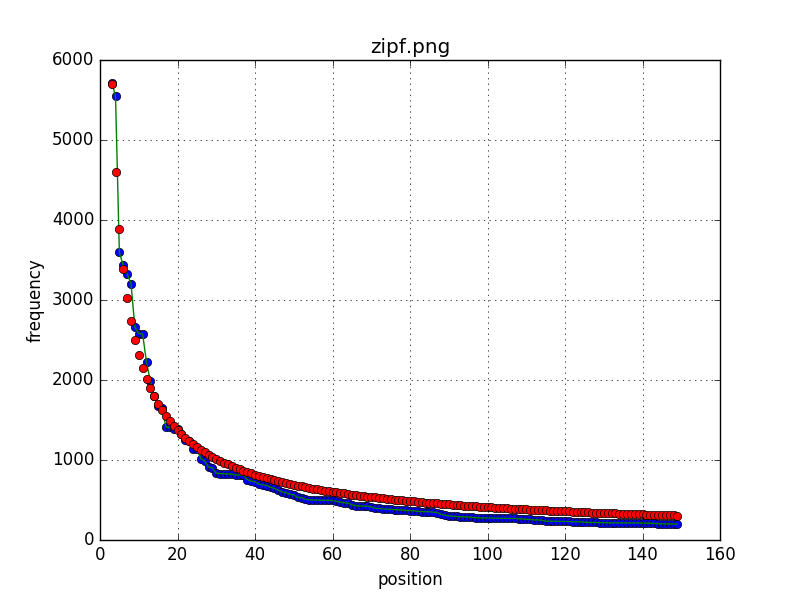
\includegraphics[scale=0.8]{pics/zipf.png}
  \caption{Зависимость частоты слова от позиции в отсортированной по
    убыванию частоты последовательности слов. Синие точки --- реальные данные,
    красные --- формула с подобранными коэффициентами.}
  \label{fig:zipf}
\end{figure}

\subsection*{Выводы}
Закон Ципфа действительно очень хорошо согласуется с реальными данными.

\end{document}

